\chapter{Planetbevægelse}
%
%
\section*{Planetbaner og excentricitet}
%
%
\begin{opgave}{Excentricitet og planetbaner}{1}
Betragt formlen for afstanden mellem to objekter i bane omkring hinanden, ligning \eqref{k-eq:Ellipse_i_polaere_koordinater} i kompendiet.
\opg Lad $\epsilon = 0$. Hvad er $r(\phi)$? Og hvilken geometrisk form er dette?
\opg Lad $\epsilon = 1$. Hvilket keglesnit fås? Hvad sker der med $r(\phi)$, når $\phi$ vokser mod $\pi$?
\opg Lad $\epsilon > 1$. Hvordan er dette tilfælde sammenlignet med det, hvor $\epsilon = 1$? Beskriv forskellene mellem disse to.\\
Hint: Undersøg grænsebetingelser.
\end{opgave}
%
%
\begin{opgave}{Halleys komet}{1} \label{opg:Halleys_komet}
Halleys komet, navngivet efter den angelske astronom Edmund Halley, kredser om Solen i en meget elliptiske bane med $\epsilon = 0,967$. Den korteste afstand, som kommeten har til Solen, er $0,59 \, \text{AU}$.
%
\opg Opstil et udtryk for den største afstand $r_{\mathrm{maks}}$ som funktion af den korteste afstand $r_{\mathrm{min}}$.
%
\opg Beregn den største afstand til Solen.\\ \\
\end{opgave}
%
%
\begin{opgave}{Excentricitet}{1}
\opg Find et udtryk for excentricitetet fra formlen udledt i opgave \ref{opg:Halleys_komet}.
%
\opg Hvad er den største og mindste værdi, som excentriciteten kan antage? Hvilke(n) type(r) bane(r) gør dette sig gældende for, og hvorfor?
\end{opgave}
%
%
%
\section*{Tolegemeproblemet}
%
%
\begin{opgave}{Ækvivalens i tolegemeproblemet}{1} \label{opg:AekvivalensITolegemeproblemet}
I beskrivelsen af tolegemeproblemet blev det konkluderet, at den fælles afstand $r(\phi)$ mellem de to objekter, kan beskrives som en ellipse, der er en funktion af vinklen $\phi$ med brændpunkt i origo. Hvis vi kigger på et system bestående kun af Jorden og Solen, så betyder dette resultat, at det er lige så gyldigt at lægge solen i brændpunktet og se Jordens ellipsebevægelse omkring Solen, som at gøre det den anden vej rundt. Hvis Jorden lægges i brændpunktet, således at Jorden sættes til at stå stille, og Solens ellipsebane omkring Jorden observeres, hvordan vil massemidtpunktet så bevæge sig rent symbolsk?
\end{opgave}
%
%
\begin{opgave}{Ækvivalens i tolegemeproblemet II}{1}
I opgave \ref{opg:AekvivalensITolegemeproblemet} blev Jorden sat som at være i brændpunktet. I denne opgave sættes massemidtpunktet i stedet i brændpunktet. Må man dette, og hvis ja, hvorfor? Hvordan vil Jordens og Solens bevægelse i dette tilfælde se ud?
\end{opgave}
%
%
%
\section*{Bevægelsesligningerne}
%
%
\begin{opgave}{Bevarelse af impulsmoment}{1} \label{opg:Bevarelse_af_impulsmoment}
I afsnittet om bevarelse af impulsmoment i kompendiet argumenterede vi for, at det samlede impulsmoment for tolegemesystemet er bevaret.\\
I denne opgave skal det samme vises, men denne gang med udgangspunkt i hvert af legemerne for sig.
%
\opg Lad origo være i massemidtpunktet for tolegemesystemet og tegn dette system, hvor legemerne (kaldet 1 og 2) er i apoapsis af deres bane, og indtegn disse baner, når der tages højde for deres relative excentricitet. Angiv også stedvektorerne for de to legemer. Tegn gerne stort, da der i senere spørgsmål skal tilføjes til denne tegning.
%
\opg Indtegn de virkende kræfter og tag højde for deres relative længder.\\[2.5mm]
%
Fra kapitlet om dynamik af roterende legemer i Analytisk Mekanik, udledte vi en ligning for kraftmomentet på et legeme, ligning \eqref{k-eq:Kraftmoment}
\begin{align*}
	\v{\tau} &= \v{r} \times \v{F} \: ,
\end{align*}
og for impulsmomentet, ligning \eqref{k-eq:L}
\begin{align*}
	\v{\ell} &= \v{r} \times \v{p} \: .
\end{align*}
%
\opg Beregn kraftmomentet for hvert af legemerne.
%
\opg Hvad fortæller de beregnede kraftmomenter om impulsmomenterne? Og hvad kan der herudfra konkluderes om systemets totale impulsmoment?
%
\opg Indtegn retningen af det totale impulsmoment på tegningen, idet hvert af legemerne bevæger sig mod uret i deres respektive baner.
\end{opgave}
%
%
\begin{figure}[h!]
	\centering
	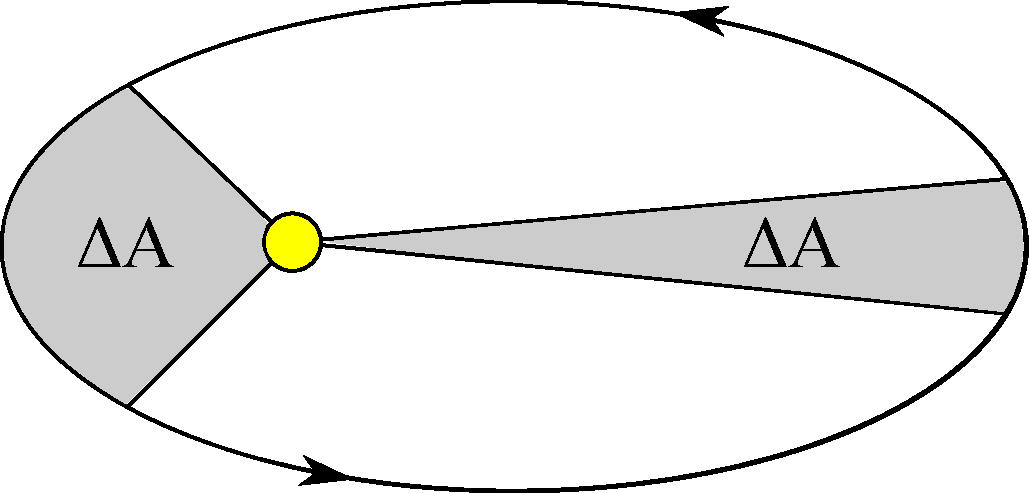
\includegraphics[width=\columnwidth]{Planetbevaegelse/Kepler2.pdf}
	\caption{Keplers 2. lov: I lige store tidsrum $\Delta t$ overstryger linjen mellem planeten og stjernen lige store arealer $\Delta A$.}
	\label{fig:Kepler2}
\end{figure}
%
\begin{opgave}{Keplers 3. lov}{2}
Keplers 2. lov beskriver, at en planet bevæger sig i sin bane, således at linjen fra stjernen til planeten, som kredser om denne, overstryger lige store arealer i lige store tidsrum, se figur \ref{fig:Kepler2}. Raten som linjen overstryger arealet med er dermed konstant, og den er givet ved
\begin{align*}
	\dif{t}{A} &= \frac{\ell}{2\mu} \: ,
\end{align*}
hvor $\ell$ er impulsmomentet og $\mu$ er den reducerede masse. Det totale areal for en ellipse er givet ved
\begin{align*}
	A &= \pi a b \: ,
\end{align*}
hvor $a$ og $b$ er hhv. den halve stor- og lilleakse.\\
Perioden for planeten er givet ved
\begin{align*}
	P &= \frac{A}{\d A / \d t} \: .
\end{align*}
%
\opg Udled ved hjælp af ovenstående og nogle formler fra kompendiet Keplers 3. lov:
\begin{align*}
	P^2 &= \frac{4\pi}{G(m_1+m_2)}a^3 \: .
\end{align*}
\end{opgave}
%
%
\begin{opgave}{Energibevarelse og excentricitet}{3}
For at finde en sammenhæng mellem excentricitet og energi betragtes en komet, der bevæger sig omkring et større objekt. Husk at energien, kompendiets ligning \eqref{k-eq:Bevaegelsesligningerne_energi}, er giver ved
\begin{align*}
	E &= \frac{1}{2}\mu v^2 + V_{\text{eff}}(r) \: .
\end{align*}
I opgaven anvendes det at
\begin{align*}
	V_{\text{eff}}(r) &= \frac{\ell^2}{2\mu r^2}-\frac{\gamma}{r} \: ,
\end{align*}
hvor $\gamma = Gm_1m_2$.
%
\opg Hvad vil kometens hastighed være, når den er tættest på objektet, altså i en afstand $r_{min}$ fra det? Og hvad vil energien så være i dette tilfælde?\\
Hint: Til at bestemme hastigheden, prøv at overvej hvilken retning, den vil have lige før $r_{min}$ samt lige efter. Husk at der kigges på et endimensionelt problem. Overvej at tegne $r$ som funktion af vinklen.
%
\opg Beregn $r_{\text{min}}$. Anvend definitionen af konstanten
\begin{align*}
	c = \frac{\ell^2}{\gamma\mu} \: .
\end{align*}
%
\opg Indsæt værdien for $r_{\text{min}}$ i udtrykket for energie, $E(r_{\text{min}})$, og bestem et udtryk for energien ud fra excentriciteten. Anvend energibevarelse til at bestemme energien til alle steder på kometens bane.
%
\opg Relater resultatet til de mulige baner. Hvis kometens totale energi er negativ, hvilken excentricitet kræves der så? Og hvordan bliver banen så? Hvad hvis energien er $0$? Eller hvis den er positiv?
\end{opgave}
%
%
%
\section*{Baneskift}
%
%
\begin{opgave}{Boostfaktor}{1}
En satellit er i kredsløb om Jorden i en cirkulær bane. Tegn den bane som fremkommer, når
\opg $\lambda > 1$.
\opg $1 > \lambda > 0$.
\opg $0 > \lambda > -1$.
\opg $\lambda < -1$.
\end{opgave}
%
%
\begin{opgave}{Boostkraft}{2}
En satellit boostes i punktet $P$ med en boostfaktor $\lambda$ for at skifte mellem to baner.
%
\opg Vis at det tidslige gennemsnit af en kraft er givet ved
\begin{align*}
	\v{F}_{av} &= \frac{\Delta \v{p}}{\Delta t} \: .
\end{align*}
%
\opg Find størrelsen af boostkraften som satellitten skal påvirkes med i løbet af boostet, som foregår over et kort tidsrum $\Delta t$.\\
Hint: Brug forskellen i impulsmoment til at finde forskellen i impuls i punktet $P$.
\end{opgave}
%
%
\begin{opgave}{Hohmannbane}{2} \label{opg:Hohmannbane}
En måde at lave et baneskift er ved brug af en Hohmannbane. Denne bane er en ellipse, som har periapsis i den ene bane og apoapsis i den anden.\\
I denne opgave betragtes en satellit, der benytter en Hohmannbane til at skifte mellem to cirkulære baner, figur \ref{fig:Hohmann}, med radius $R_1$ og $R_3 = 2R_1$.
%
\opg I hvilket punkt, $P$ eller $P'$, har Hohmann-banen hhv. periapsis og apoapsis.
%
\opg Beregn boostfaktoren $\lambda$ for satellittens boost ved punktet $P$.\\
Hint: Opstil et udtryk for $R_3$ ved $R_1$.\\
%
\opg Beregn boostfaktoren $\lambda'$ for satellittens boost ved punktet $P'$.\\
Hint: Betragt sammenfaldet mellem de to baner i $P'$.
%
\opg Brug impulsmomentbevarelse til at udtrykke satelittens hastighed $v_3$ efter begge boosts ved dens hastighed $v_1$ før boostene.
\end{opgave}
%
%
\begin{figure}[h!]
	\centering
	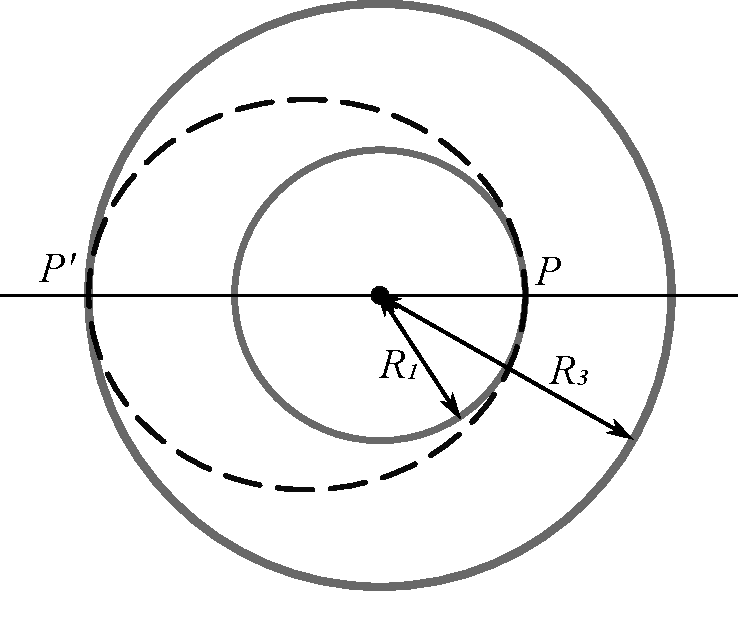
\includegraphics[width=\columnwidth]{Planetbevaegelse/Hohmann.pdf}
	\caption{To cirkulære baner (grå) og en Hohmannbane (stiplet) til at skifte mellem banerne.}
	\label{fig:Hohmann}
\end{figure}
%
%
\begin{opgave}{Hohmannbane II}{2}
En satellit vil nu gerne i to steps skifte mellem tre cirkulære baner. I første step skifter den fra bane A til C via Hohmannbanen 1, og i andet step skifter den fra bane C til bane B via Hohmannbanen 2. Se figur \ref{fig:Hohmann2}. Bane A har radius $R_A$, bane B har radius $R_B = 3R_A$ og bane C har radius $R_C = 1,5 R_B = 4,5 R_A$. Beregn følgende boostfaktorer.
%
\opg $\lambda_1$ i punktet $P$ for at skifte fra bane A til Hohmannbanen 1.
\opg $\lambda_1'$ i punktet $P'$ for at skifte fra Hohmannbanen 1 til bane C.
\opg $\lambda_2$ i punktet $Q$ for at skifte fra bane C til Hohmanbanen 2.
\opg $\lambda_2'$ i punktet $Q'$ for at skifte fra Hohmannbanen 2 til bane B.
%
\opg Hvad gør sig gældende for formen af boostfaktorerne $\lambda_1$ og $\lambda_2$ samt $\lambda_1'$ og $\lambda_2'$?\\
Hint: Generaliser boostfaktorerne.
\end{opgave}
%
\begin{figure}[h!]
	\centering
	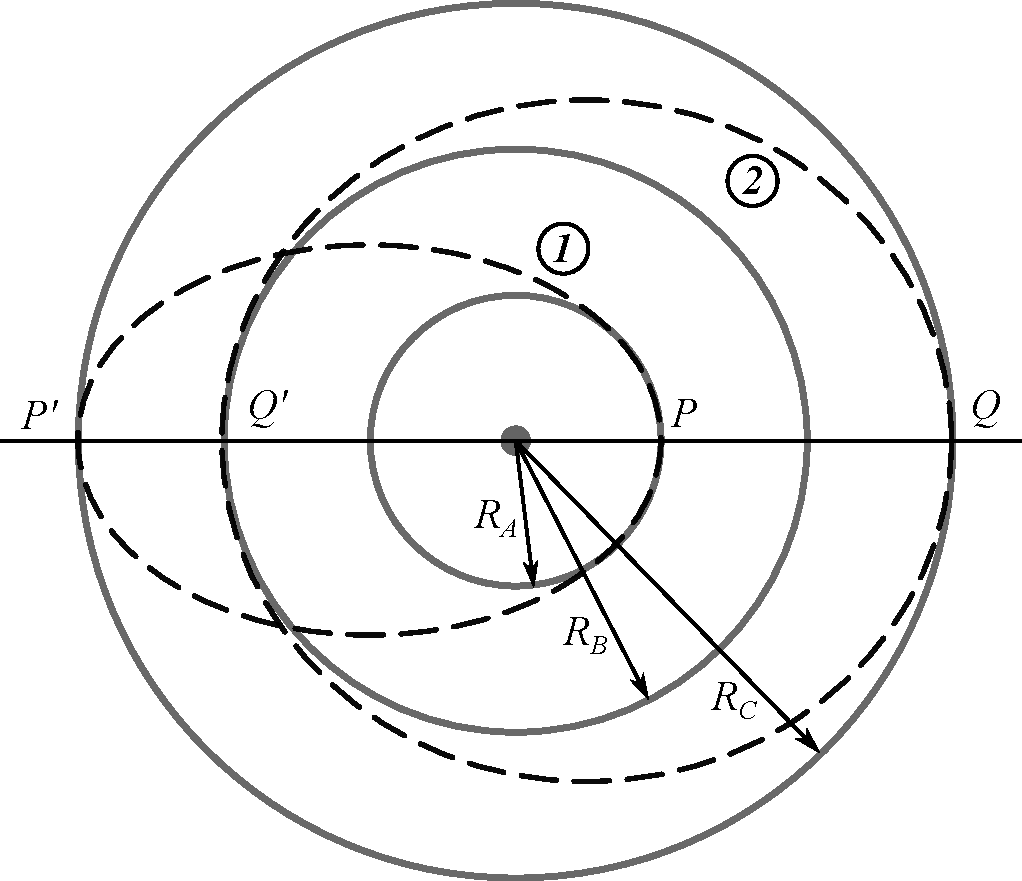
\includegraphics[width=\columnwidth]{Planetbevaegelse/Hohmann2.pdf}
	\caption{Tre cirkulære baner (grå) og to Hohmannbaner (stiplede) til at skifte mellem banerne.}
	\label{fig:Hohmann2}
\end{figure}